\newpage
\section{Durchführung}
\label{sec:Durchführung}
Am Anfang des Versuch werden die zwei Kugeln gewogen
und mehrmals vermessen. Zuerst wird der Versuch mit
der kleineren Kugel durchgeführt, dafür wird die
Röhre des Kugelfall-Viskosimeters siehe Abbildung \ref{abb:visko} mit destilliertem Wasser und der kleineren Kugel
aufgefüllt und, ohne Luft einzuschließen, verschlossen.
\begin{figure}
 \centering
 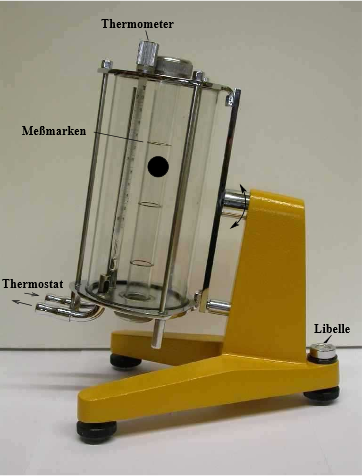
\includegraphics[width=0.5\textwidth]{bild.PNG}
\caption{Die Abblidung zeigt das verwendete Kugelfall-Viskosimeter nach Höppler.\cite{sample}}
\label{abb:visko}
\end{figure}
Die Messung besteht darin, dass die Zeit mehrmals
gemessen wird, die die Kugel in der Flüssigkeit benötigt,
um eine makierte Strecke zu sinken, ist die Kugel unten angekommen
lässt sich die Röhre um 180° drehen und die Messung wiederholen.
Die kleinere Kugel wird nun gegen die größere Kugel
ausgetauscht und mit dieser wird ebenfalls die Messung
durchgeführt. Nun wir durch ein Thermostat
die Temperatur des destillierten Wassers verändert,
wieder wird die Messung wie oben beschrieben,
für unterschiedliche
Temperaturen, wiederholt.
